\documentclass[a4paper, 12pt]{report}

\usepackage{titlesec}  % Allow the chapter/section heading settings to be fine-tuned.  Needs to come before bidi, in polyglossia.
\usepackage{polyglossia}  % multilingual support
\usepackage{longtable}  % tables that carry across multiple pages
\usepackage[x11names]{xcolor}  % can't use color with polyglossia

%--------------------------------
%%% Font definitions %%%
%--------------------------------

% Note that these definitions malfunction if used in \chapter{}.
\defaultfontfeatures{Mapping=tex-text}
\setmainfont{Charis SIL}  % Set the default font for the document. = \setdefaultfont
% Footnotes will by default also use this font -- http://tex.stackexchange.com/questions/4779/how-to-change-font-family-in-footnote).
\defaultfontfeatures{Scale=MatchLowercase}  % needs to be below main font declaration

\setsansfont{Liberation Sans}
\setmonofont{DejaVu Sans Mono}

\setmainlanguage{english}
\setotherlanguage{arabic}

\newfontfamily\arabicfont[Script=Arabic, Scale=2]{Scheherazade} % Arabic transcription -- coloured black, double size.
% One font needs to be called \arabicfont in order for XeTeX to load Arabic-related hyphenation and other stuff.
%  The default \textarabic will use this \arabicfont.  Use the \begin{Arabic} ..... \end{Arabic} environment for longer stretches (eg paras).
% Use \textarabic{\aemph{با}} to give overline emphasis.
% Omitting Script=Arabic for Amiri or Granada will mean that letters are written in their standalone forms, not connected.  (Omitting Script=Arabic for Scheherazade seems to cause no problem, though.)

\newfontfamily\citationfont[Script=Arabic, Scale=1.5]{Scheherazade}  % Citations, or stand-alone Arabic script in the middle of Roman script -- coloured black, one-and-a-half size.
\newcommand\AS[1]{{\citationfont\RLE{#1}}}
% \RLE (from the bidi package, which polyglossia loads automatically) is to allow multiple words of Arabic to be written right-to-left -- if omitted, each word in the sequence will be written RTL, but the sequence as a whole will be written LTR.

%You can either, as above, define a new \fontfamily, and then use it in a \newcommand, or you can, as below, include the font in the \newcommand by calling \fontspec directly.

\newcommand\Atitle[1]{{\fontspec[Script=Arabic, Scale=2]{GranadaKD}\RLE{#1}}}  % Arabic transcription for titles - uses a version of Granada which has been extended to include glyphs for Swahili.

\newcommand\Am[1]{{\fontspec[Script=Arabic]{Amiri}\RLE{#1}}} % Examples using Amiri --  if using Scheherazade's default scale, set Scale=0.8 here.

%\newfontfamily\translitfont[Scale=1, Color=666666]{Linux Biolinum O}
%\newcommand\Tr[1]{{\translitfont\RLE{#1}}}
\newcommand\Tr[1]{{\fontspec[Scale=1, Color=666666]{Linux Biolinum O}#1}}   %  Transliteration -- Biolinum handles diacritics well.  Coloured grey, slightly less than normal size.
% Scale=1 is required because of Scale=MatchLowercase - otherwise the size is too large.
\newcommand\Trb[1]{{\fontspec[Scale=1, Color=0000BB]{Linux Biolinum O}#1}} 

\newcommand\In[1]{{\fontspec[Scale=1, Color=blue]{Linux Biolinum O}#1}}  % Epenthetic letters in the transliteration -- coloured blue, normal size.

\newcommand\Swa[1]{{\fontspec[Color=00BB33, Scale=1]{Linux Biolinum O}#1}}  % Standard spelling -- coloured green, normal size.

\newcommand\E[1]{{\fontspec[Scale=0.9, Color=333333]{Liberation Serif Italic}#1}}  % English translation layer -- coloured grey, slightly less than normal size.

\newcommand\Eit[1]{{\fontspec{Liberation Serif Italic}#1}}  % English italics.

\newcommand\FN[1]{{\fontspec[Color=00BB33]{Liberation Serif Italic}#1}} % Standout type in footnotes -- coloured green, normal size.

% Older versions:
% \newfontfamily{\Tr}[Scale=0.9, Color=00BB33]{Linux Biolinum O}
% This can be used as \Tr{text}.  But this will change the font outside the argument until the end of that stretch.
% This doesn't show up in the poemlines, because they are self-contained, but it does show up in connected text.
% To avoid this, and have the font only changed within the argument, use \newcommand as above.
% Though you can also enclose \Tr in braces to limit it: {\Tr{}}

%----------------------------------------
%%% End of font definitions %%%
%----------------------------------------

%--------------------------------
%%% Colour definitions %%%
%--------------------------------

\definecolor{mygreen}{RGB}{0, 187, 50}

%----------------------------------------
%%% End of font definitions %%%
%----------------------------------------

  % Bring in the font definitions.

\usepackage{graphicx}  % Allows images to be inserted.
\usepackage{pdfpages}

\usepackage{marginnote}
\renewcommand*{\marginfont}{\color{red}\sffamily}

\usepackage{csquotes}
% \usepackage{natbib}
\usepackage[backend=biber, style=authoryear]{biblatex}
\addbibresource{bib/andika.bib}

\interfootnotelinepenalty=10000 % prevents the footnote from breaking across pages
% http://tex.stackexchange.com/questions/32208/footnote-runs-onto-second-page

% Thanks to Manas Tungare (http://manas.tungare.name/software/latex) for these settings.
\setlength{\paperwidth}{210mm}
\setlength{\paperheight}{297mm}

\setlength{\textwidth}{160mm}
\setlength{\textheight}{247mm}

\setlength{\evensidemargin}{1in}
\setlength{\oddsidemargin}{0in}
\setlength{\topmargin}{-0.5in}

% \renewcommand\thefootnote{\textcolor{red}{\arabic{footnote}}}  % Alter the colour of the footnote markers - thanks to Gonzalo Medina (http://tex.stackexchange.com/questions/26693/change-the-color-of-footnote-marker-in-latex#26696).

\usepackage{url}  % Use urls in text and captions with sensible linewrap.  Can't use [obeyspaces] - this option clashes with biblatex.
% \urlstyle{rm}  % Set urls in roman.

\titleformat{\chapter}[display]{\normalfont\large}{\bfseries\chaptertitlename\ \thechapter}{10pt}{\large\itshape}[\vspace{2ex}\titlerule\vspace{2ex}]  % 10pt is the space between chapter and chapter name.  [display] sets the chapter and chapter name on separate lines.  The square brackets at the end draw a line under each chapter name, with 2ex gap from the name.
\titlespacing{\chapter}{0pt}{0pt}{10pt}  % First is indent from the side, second is length down from the top, third is gap between heading and text.

% \pagenumbering{gobble}  % Suppress page numbering.

% ===== Endnotes =====
% Uncomment the following two lines to get endnotes instead of footnotes.
% Remember to uncomment the three lines in andika/db/output_pdf.php as well.
% \usepackage{endnotes}
% \let\footnote=\endnote
% ==================

\begin{document}


\begin{center}
\Atitle{أُتٖينْزِ وَ رَاسِ الغُولِ} \\
\E{Mtungaji: Mgeni bin Faqihi, c. 1850} \\
\vspace{8mm}
\end{center}

\begin{small}
This is a transcription of the MS sample included in Leo van Kessel's edition of \FN{Utenzi wa Rasi 'lGhuli} by Mgeni  bin  Faqihi (Tanzania Publishing House, Dar Es Salaam, 1979).  This was composed around 1850, and at over 4,500 stanzas is the longest Swahili ballad in existence.  The editor used four MS, but which one the sample was taken from is not specified - comparing the published text (the green line below) with the MS text above it shows a number of differences, and one stanza from the MS (between 2285 and 2286) does not appear in the published text.  The copyist of this MS writes only 3 vowels, uses \textit{ain} with dot to represent `ng[w]', and tends not to mark nasalised or labialised consonants (e.g.  \textarabic{وَكِتُزَ}, \Eit{wakitunza}, 2283a; \textarabic{كَتُمَ}, \Eit{kwa Tumwa}, 2285c).
\end{small}
\vspace{8mm}



\begin{longtable}{rrl} 

\makebox[8cm][r]{} & & \makebox[8cm][r]{} \\ 

\textarabic{نِكِغَ كُنَ جَبَلِ} & \textarabic{نَلِغُ حِلُ ثَقِلِ} & \textarabic{٢٢٧٦} \\* 
\Tr{nikiḡa kuna jabali} & \Tr{naliḡu ḥilu thaqili} &  \Tr{2276b/a} \\* 
\multicolumn{2}{r}{\Swa{na lango hili thaqili * kana pande la jabali}} & \Swa{2276a/b} \\* 
\multicolumn{2}{r}{\E{ }} & \\ 
\textarabic{زَحَدِدِ نَصِفُرِ} & \textarabic{لِفُغَ كَسِلِ سِلِ} &  \\* 
\Tr{zaḥadidi naṣifuri} & \Tr{lifuḡa kasili sili} &  \Tr{2276d/c} \\* 
\multicolumn{2}{r}{\Swa{lifungwa kwa silisili * za hadidi na sufuri}} & \Swa{2276c/d} \\* 
\multicolumn{2}{r}{\E{ }} & \\ 
\\[8mm] 

\textarabic{وَسِمَامِ وِنْيِ قُوَ} & \textarabic{وِدَبُ وَكِفُغُوَ} & \textarabic{٢٢٧٧} \\* 
\Tr{wasimāmi winyi quwa} & \Tr{widabu wakifuḡuwa} &  \Tr{2277b/a} \\* 
\multicolumn{2}{r}{\Swa{wendepo wakifungua * wasimame wenye quwa}} & \Swa{2277a/b} \\* 
\multicolumn{2}{r}{\E{ }} & \\ 
\textarabic{سَبْعِنِ مَكُفَرِ} & \textarabic{وَوُمِ وَسِوُتُوَ} &  \\* 
\Tr{sabʾini makufari} & \Tr{wawumi wasiwutuwa} &  \Tr{2277d/c} \\* 
\multicolumn{2}{r}{\Swa{waume wasiotuwa * sabiini makufari}} & \Swa{2277c/d} \\* 
\multicolumn{2}{r}{\E{ }} & \\ 
\\[8mm] 

\textarabic{كُفُغَ هَوَحِمِلِ} & \textarabic{وَتُ وَكِوَ قَلِلِ} & \textarabic{٢٢٧٨} \\* 
\Tr{kufuḡa hawaḥimili} & \Tr{watu wakiwa qalili} &  \Tr{2278b/a} \\* 
\multicolumn{2}{r}{\Swa{watu wakiwa qalili * kufunga hawahimili}} & \Swa{2278a/b} \\* 
\multicolumn{2}{r}{\E{ }} & \\ 
\textarabic{مُشَبَهَ وَحَجَرِ} & \textarabic{كَلَغُ كُوَ ثَقِلِ} &  \\* 
\Tr{mushabaha waḥajari} & \Tr{kalaḡu kuwa thaqili} &  \Tr{2278d/c} \\* 
\multicolumn{2}{r}{\Swa{kwa lango kuwa thaqili * mshabaha wa hajari}} & \Swa{2278c/d} \\* 
\multicolumn{2}{r}{\E{ }} & \\ 
\\[8mm] 

\textarabic{تِنَ ِدِكَوَثِقِ} & \textarabic{مَلْعُوُنِ مُنَفِقِ} & \textarabic{٢٢٧٩} \\* 
\Tr{tina idikawathiqi} & \Tr{malʾuwuni munafiqi} &  \Tr{2279b/a} \\* 
\multicolumn{2}{r}{\Swa{maleuni mnafiqi * na nde amewathiqi}} & \Swa{2279a/b} \\* 
\multicolumn{2}{r}{\E{ }} & \\ 
\textarabic{كَزِعَ دَوِمَدَرِ} & \textarabic{اَمَتِبَ نَحَدَقِ} &  \\* 
\Tr{kaziʾa dawimadari} & \Tr{amatiba naḥadaqi} &  \Tr{2279d/c} \\* 
\multicolumn{2}{r}{\Swa{ametimba na khandaqi * amezinga mdawari}} & \Swa{2279c/d} \\* 
\multicolumn{2}{r}{\E{ }} & \\ 
\\[8mm] 

\textarabic{مَبَنَيِ تَبَيِنِ} & \textarabic{نَخَدَقِ فَهَمُنِ} & \textarabic{٢٢٨٠} \\* 
\Tr{mabanayi tabayini} & \Tr{nakhadaqi fahamuni} &  \Tr{2280b/a} \\* 
\multicolumn{2}{r}{\Swa{na khandaqi fahamuni * mpanaye tabaini}} & \Swa{2280a/b} \\* 
\multicolumn{2}{r}{\E{ }} & \\ 
\textarabic{كَذِرَعَ زَمَكُفَرِ} & \textarabic{نِذِرَعَ عِشِرِنِ} &  \\* 
\Tr{kadhiraʾa zamakufari} & \Tr{nidhiraʾa ʾishirini} &  \Tr{2280d/c} \\* 
\multicolumn{2}{r}{\Swa{ni dhiraa ishirini * kwa dhiraa za makufari}} & \Swa{2280c/d} \\* 
\multicolumn{2}{r}{\E{ }} & \\ 
\\[8mm] 

\textarabic{مُلِ دَنِ يَحُصُنِ} & \textarabic{اَكِكِلِتِ لَعِنِ} & \textarabic{٢٢٨١} \\* 
\Tr{muli dani yaḥuṣuni} & \Tr{akikiliti laʾini} &  \Tr{2281b/a} \\* 
\multicolumn{2}{r}{\Swa{akikeleti laini * mle ndani ya husuni}} & \Swa{2281a/b} \\* 
\multicolumn{2}{r}{\E{ }} & \\ 
\textarabic{يَأدِ وَسِفِكِرِ} & \textarabic{وَلِوَ كُطُمَعِنِ} &  \\* 
\Tr{yadi wasifikiri} & \Tr{waliwa kuṭumaʾini} &  \Tr{2281d/c} \\* 
\multicolumn{2}{r}{\Swa{wakiwa kutumaini * ya nde wasifikiri}} & \Swa{2281c/d} \\* 
\multicolumn{2}{r}{\E{ }} & \\ 
\\[8mm] 

\textarabic{خِ زِكَفِكَ} & \textarabic{وَكِكَعَ مُشِرِكَ} & \textarabic{٢٢٨٢} \\* 
\Tr{khi zikafika} & \Tr{wakikaʾa mushirika} &  \Tr{2282b/a} \\* 
\multicolumn{2}{r}{\Swa{wakikaa mushirika * siku nyingi zikafika}} & \Swa{2282a/b} \\* 
\multicolumn{2}{r}{\E{ }} & \\ 
\textarabic{مُكُوُ وَلاَ صَغِرِ} & \textarabic{بَسِوِ مُتُ كُتُكَ} &  \\* 
\Tr{mukuwu wala ṣaḡiri} & \Tr{basiwi mutu kutuka} &  \Tr{2282d/c} \\* 
\multicolumn{2}{r}{\Swa{pasiwe mtu kutoka * mkuu wala saghiri}} & \Swa{2282c/d} \\* 
\multicolumn{2}{r}{\E{ }} & \\ 
\\[8mm] 

\textarabic{كُوَطُلِيَ مَقَامُ} & \textarabic{وَكِتُزَ اِسِلَامُ} & \textarabic{٢٢٨٣} \\* 
\Tr{kuwaṭuliya maqāmu} & \Tr{wakituza isilāmu} &  \Tr{2283b/a} \\* 
\multicolumn{2}{r}{\Swa{wakitunza islamu * kuwatwalia maqamu}} & \Swa{2283a/b} \\* 
\multicolumn{2}{r}{\E{ }} & \\ 
\textarabic{كِدَ وَنَ نَكُفَرِ} & \textarabic{بَبَلِ وَكَعَزِمُ} &  \\* 
\Tr{kida wana nakufari} & \Tr{babali wakaʾazimu} &  \Tr{2283d/c} \\* 
\multicolumn{2}{r}{\Swa{kwa papo wakiazimu * kwenda wana na kufari}} & \Swa{2283c/d} \\* 
\multicolumn{2}{r}{\E{ }} & \\ 
\\[8mm] 

\textarabic{وَكِبُ كُتَقَرَبُ} & \textarabic{وَكَوِدِيَ كِلَابُ} & \textarabic{٢٢٨٤} \\* 
\Tr{wakibu kutaqarabu} & \Tr{wakawidiya kilābu} &  \Tr{2284b/a} \\* 
\multicolumn{2}{r}{\Swa{wakiwendea kilabu * walipo kutaqarabu}} & \Swa{2284a/b} \\* 
\multicolumn{2}{r}{\E{ }} & \\ 
\textarabic{كَنَ وِغُ لَمَطَرِ} & \textarabic{وَكَبِغَ كَنِشَبُ} &  \\* 
\Tr{kana wiḡu lamaṭari} & \Tr{wakabiḡa kanishabu} &  \Tr{2284d/c} \\* 
\multicolumn{2}{r}{\Swa{wakipigwa kwa nishabu * kana wingu la matari}} & \Swa{2284c/d} \\* 
\multicolumn{2}{r}{\E{ }} & \\ 
\\[8mm] 

\textarabic{صَحَبَ وَكِوُمِيَ} & \textarabic{مِشَرِ يِكُوَغِيَ} & \textarabic{٢٢٨٥} \\* 
\Tr{ṣaḥaba wakiwumiya} & \Tr{mishari yikuwaḡiya} &  \Tr{2285b/a} \\* 
\multicolumn{2}{r}{\Swa{mishale ikawangia * sahaba wakiumia}} & \Swa{2285a/b} \\* 
\multicolumn{2}{r}{\E{ }} & \\ 
\textarabic{نَمَجَرَحِ كَثِرِ} & \textarabic{كَتُمَ وَكَرِجِيَ} &  \\* 
\Tr{namajaraḥi kathiri} & \Tr{katuma wakarijiya} &  \Tr{2285d/c} \\* 
\multicolumn{2}{r}{\Swa{kwa tumwa wakirejea * na majeruhi kathiri}} & \Swa{2285c/d} \\* 
\multicolumn{2}{r}{\E{ }} & \\ 
\\[8mm] 

\textarabic{مِثَرِ كُوَ خَسِرِ} & \textarabic{اَكِتَرَمَ بَشِرِ} & \\* 
\Tr{mithari kuwa khasiri} & \Tr{akitarama bashiri} &  \Tr{b/a} \\* 
\multicolumn{2}{r}{\Swa{akitarama bashiri * mithari kuwa hasiri}} & \Swa{a/b} \\* 
\multicolumn{2}{r}{\E{ }} & \\ 
\textarabic{اَكِتُوَ مَشَوُرِ} & \textarabic{بَبَلِ اَكِفِصِرِ} &  \\* 5
\Tr{akituwa mashawuri} & \Tr{babali akifiṣiri} &  \Tr{d/c} \\* 
\multicolumn{2}{r}{\Swa{babali akifisiri * akituwa mashawuri}} & \Swa{c/d} \\* 
\multicolumn{2}{r}{\E{ }} & \\ 
\\[8mm] 

\textarabic{كُوَبِيَ اَصْحَبُ} & \textarabic{اَكِتَمُكَ حَبِبُ} & \textarabic{٢٢٨٦} \\* 
\Tr{kuwabiya aṣḥabu} & \Tr{akitamuka ḥabibu} &  \Tr{2286b/a} \\* 
\multicolumn{2}{r}{\Swa{akitamka habibu * kuwambia asahabu}} & \Swa{2286a/b} \\* 
\multicolumn{2}{r}{\E{ }} & \\ 
\textarabic{كُفَرِ كُوَظفر} & \textarabic{مُتَكَبُ يَصَوَبُ} &  \\* 
\Tr{kufari kuwaẓfr} & \Tr{mutakabu yaṣawabu} &  \Tr{2286d/c} \\* 
\multicolumn{2}{r}{\Swa{mtakapo ya sawabu * kufari kuwadhifiri}} & \Swa{2286c/d} \\* 
\multicolumn{2}{r}{\E{ }} & \\ 
\\[8mm] 

\end{longtable} 

\newpage

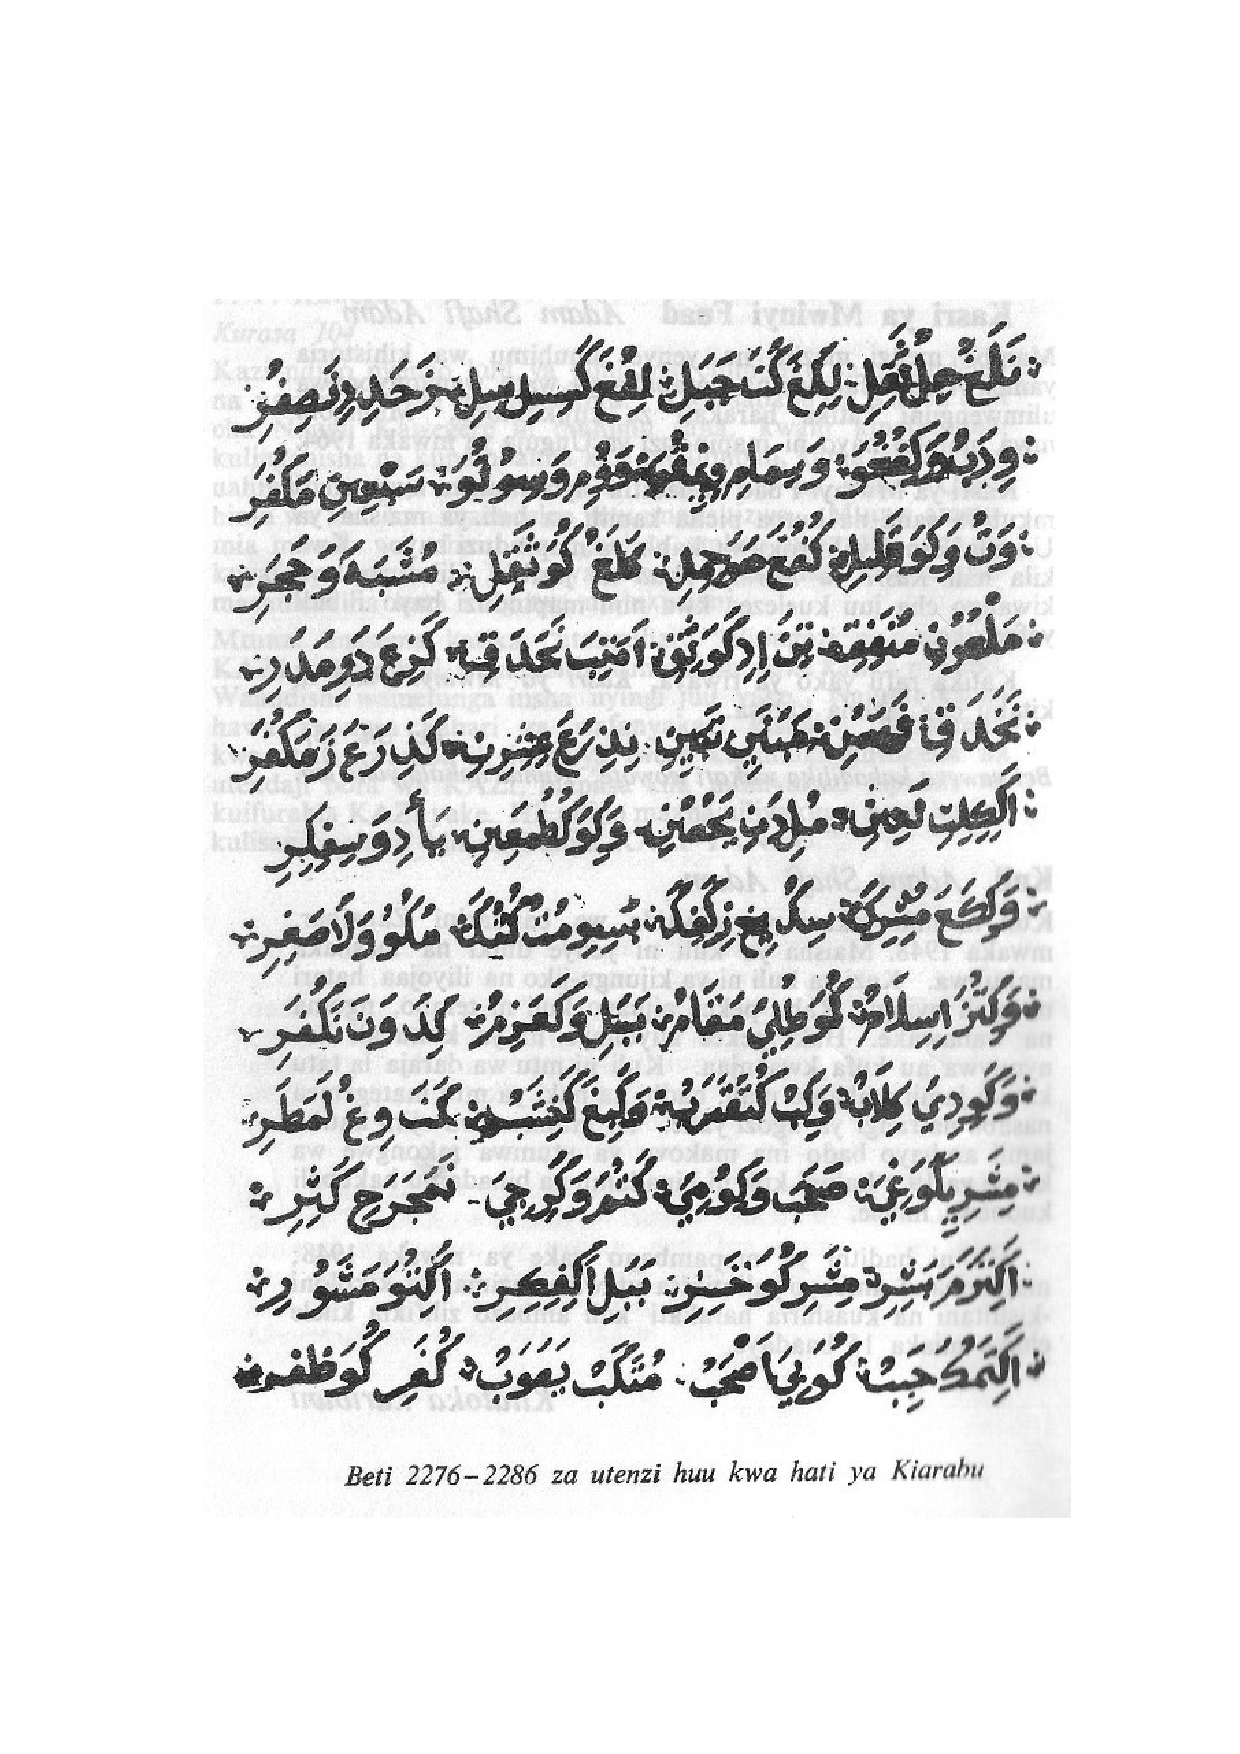
\includepdf[pages={ - }, pagecommand={}]{db/outputs/rasilghuli/MS.pdf}

\renewcommand{\bibname}{References} 
\begingroup 
\printbibliography 
\endgroup 

\end{document}
